\documentclass[10pt,landscape]{article}
\usepackage{multicol}
\usepackage{xcolor}
\usepackage{calc}
\usepackage{ifthen}
\usepackage[landscape]{geometry}
\usepackage{hyperref}
\usepackage{graphicx}
\usepackage{amsmath,amssymb}
\usepackage{algorithm2e}
\usepackage{float}
\usepackage{ragged2e}
\usepackage{enumitem}
% \usepackage{xeCJK}

\geometry{top=1cm,left=1cm,right=1cm,bottom=1cm}
% disable header/footer
\pagestyle{empty}
% make section commands use less space
\makeatletter
\renewcommand{\section}{\@startsection{section}{1}{0mm}%
    {-1ex plus -.5ex minus -.2ex}%
    {0.5ex plus .2ex}%x
    {\normalfont\large\bfseries}}
\renewcommand{\subsection}{\@startsection{subsection}{2}{0mm}%
    {-1explus -.5ex minus -.2ex}%
    {0.5ex plus .2ex}%
    {\normalfont\normalsize\bfseries}}
\renewcommand{\subsubsection}{\@startsection{subsubsection}{3}{0mm}%
    {-1ex plus -.5ex minus -.2ex}%
    {1ex plus .2ex}%
    {\normalfont\small\bfseries}}
\setlist{nosep} % or \setlist{noitemsep} to leave space around whole list
% wrappable brace text
\newlength\ubwidth
\newcommand\parunderbrace[2]{\settowidth\ubwidth{$#1$}\underbrace{#1}_{\parbox{\ubwidth}{\scriptsize\RaggedRight#2}}}
\newcommand\paroverbrace[2]{\settowidth\ubwidth{$#1$}\overbrace{#1}^{\parbox{\ubwidth}{\scriptsize\RaggedRight#2}}}

\makeatother

% BibTeX command
\def\BibTeX{{\rm B\kern-.05em{\sc i\kern-.025em b}\kern-.08em
    T\kern-.1667em\lower.7ex\hbox{E}\kern-.125emX}}
% no section numbers
\setcounter{secnumdepth}{0}

\setlength{\parindent}{0pt}
\setlength{\parskip}{0pt plus 0.5ex}

\DeclareMathOperator*{\argmax}{argmax}
% -----------------------------------------------------------------------

\begin{document}
\raggedright
\footnotesize
\begin{multicols}{3}
% multicol parameters
%\setlength{\columnseprule}{0.25pt}
\setlength{\premulticols}{1pt}
\setlength{\postmulticols}{1pt}
\setlength{\multicolsep}{1pt}
\setlength{\columnsep}{2pt}

\newcommand\pro{\item[$+$]}
\newcommand\con{\item[$-$]}
\newcommand\red{\textcolor{red}}

\begin{center}
    \Large{Reinforcement Learning (RL)} \\ % Cheat Sheet
\end{center}

\section{Symbols}

\begin{multicols}{2}
\begin{description}
    % https://en.wikipedia.org/wiki/List_of_mathematical_symbols
    % https://en.wikipedia.org/wiki/List_of_mathematical_symbols_by_subject
    % https://en.wikipedia.org/wiki/Notation_in_probability_and_statistics

    % \item[$$] 
    % \item[$lowercase$]
    % scalar / part
    % \item[$uppercase$]
    % space / total / function / matrix
    % \item[$bold$]
    % vector
    % \item[$blackboard bold$]
    % set
    \item[$a$]
    action %, arm (multi-armed bandit problem)
    \item[$A$]
    advantage
    \item[$\alpha$]
    learning rate, step size
    \item[$b$]
    bandit, baseline estimate %, bias
    \item[$c$]
    cost, context (= state)
    \item[$d$]
    difference error
    \item[$\Delta$]
    difference
    \item[$D$]
    replay buffer
    % \item[$\partial$]
    % partial derivative
    \item[$E$]
    eligibility trace % error
    % \item[$\mathbb{E} / E$]
    % expected value
    \item[$\epsilon$]
    exploration rate ($0 \sim 1$)
    % \item[$f$]
    % function
    \item[$\Phi$]
    state transition function
    \item[$g$]
    gain % (reward over time) %, target
    \item[$\gamma$]
    discount factor
    \item[$\nabla$]
    gradient % (spacial derivative)
    \item[$H$]
    horizon
    % \item[$i$]
    % this round
    % \item[$j$]
    % next round
    \item[$J$]
    expected return % (see loss)
    % \item[$k$]
    % some amount
    \item[$L$]
    loss / regret % expected (squared) loss % (see return)
    \item[$\lambda$]
    trace decay ($0 \sim 1$)
    % \item[$m$]
    % momentum % amount, matrix rows
    % \item[$\mu$]
    % mean
    % \item[$n$]
    % count
    % \item[$\mathbb{N}$]
    % natural number space
    % \item[$O / \Omega$]
    % order of magnitude
    % \item[$p$]
    % probability ($0 \sim 1$)
    \item[$Pr$]
    transition distribution
    \item[$\pi$]
    policy ($state \rightarrow action$)
    % \item[$\Pi$]
    % product
    \item[$q$]
    quality
    \item[$r$]
    reward
    \item[$R$]
    return
    % \item[$\rho$]
    % regret
    % \item[$\mathbb{R}$]
    % real number space
    \item[$s$]
    state
    % \item[$\sigma$]
    % standard deviation
    % \item[$\Sigma$]
    % sum
    \item[$t$]
    time % (sub), target value (given)
    \item[$\tau$]
    trajectory
    \item[$\theta$]
    parameter weight % (learning target) %, small positive number (iteration)
    % \item[$\theta_{i}^{-}$]
    % target network (time i-1)
    % \item[$u$]
    % user
    % \item[$U$]
    % ??? (DQN replay buffer)
    \item[$v$]
    value
    % \item[$vm$]
    % variance momentum
    \item[$w$]
    weight %, winning probability
    % \item[$x$]
    % observation
    \item[$y$]
    target / prediction %, output
    \item[$_\ast$]
    optimal
    \item[$'$]
    next / derivative
    \item[$\hat{}$]
    estimation
    \item[$\Vert\Vert$]
    vector norm
\end{description}
\end{multicols}

\section{Agent-Environment Interface}
\includegraphics[width=\linewidth]{./images/Agent-Environment.png}

\section{General model}
\begin{enumerate}
    \item the \emph{agent} at each time step $t$ receives a representation of the environment's \emph{state} $S_t \in S$
    \item it selects an action $A_t \in A(s)$
    \item from its action the agent receives a \emph{reward} $R_{t + 1} \in R \in \mathbb{R}$
\end{enumerate}

\section{General challenges}
\begin{itemize}
    \item choosing the right \emph{Representation} of the problem / state
    \item \emph{Generalization} beyond the cases trained on
    \item \emph{Temporal Credit Assignment}: what caused this outcome?
    \item balance \emph{Exploitation} vs \emph{Exploration} (short vs long term)
\end{itemize}

\section{Concepts (no state)}

\begin{equation}
    \begin{array}{l l}
        \underbrace{a}_\text{state} &\in \underbrace{A}_\text{finite set of actions}\\
        \underbrace{R}_\text{return} &= \underbrace{\sum_{t = 0}^{\overbrace{H}^\text{horizon ($\infty$?)}} r_t}_\text{total \emph{reward} over time}\\
        \underbrace{G_t}_\text{gain} &= \underbrace{
            \sum_{k = 0}^{H} \red{\overbrace{\gamma^k}^\text{discount factor}} r_{t + k + 1}
        }_\text{total \red{discounted} reward over time}\\
        \underbrace{L}_\text{regret} &= \underbrace{\overbrace{G^\ast}^\text{optimal gain} - \overbrace{G_\pi}^\text{gain under policy}}_\text{gain missed under policy}\\ %loss / 
    \end{array}
\end{equation}

\section{\href{https://en.wikipedia.org/wiki/Multi-armed_bandit}{Bandit algorithms}}

\begin{itemize}
    \item \emph{multi-armed bandit problem}: which slot arm gives most?
    \item no notion of state!
    \item this leaves just \emph{exploration vs exploitation}
\end{itemize}

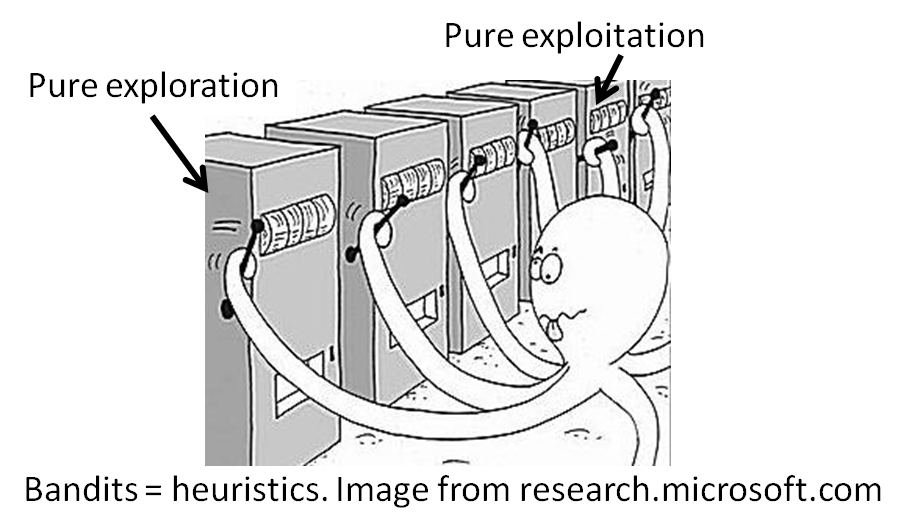
\includegraphics[width=\linewidth]{./images/bandit.png}

\begin{equation}
    \begin{array}{l l}
        \underbrace{n_{a}}_\text{action's use count} &= \underbrace{\sum_{t=0}^T \begin{cases}
            1 & a_t = a\\
            0 & \text{otherwise}
        \end{cases}}_\text{tries for action so far}\\
        \underbrace{\hat{r}_{a}}_\text{action's expected reward} &= \underbrace{\sum_{t}^a \frac{r_{t}}{n_{a}}}_\text{average action reward so far}\\
    \end{array}
\end{equation}

\subsection{\href{https://en.wikipedia.org/wiki/Greedy_algorithm}{Greedy}}

\begin{itemize}
    \item 100\% exploitation
    \item wants to pick best arm but won't know enough
    \con if 1st arm ok won't try others (stuck in local optimum)
\end{itemize}

\begin{equation}
    \begin{array}{l l}
        \underbrace{a_{t}}_\text{action at time $t$} &= \underbrace{\argmax\limits_{a \in A} \hat{r}_{a}}_\text{action with max expected reward}\\
        \underbrace{L_T}_\text{total regret}
            % &\underbrace{\propto}_\text{is proportional to}
            &\propto
            \underbrace{O(n)}_\text{order of magnitude \emph{linear} to the number of actions}\\
    \end{array}
\end{equation}

\subsection{Optimistic-Greedy}
\begin{itemize}
    % \item param $R$: initial $\hat{r}_{a}$ (large)
    \item like greedy but large initial $\hat{r}_{a}$
    \pro tries all
    \con no 2nd chance for arms unlucky on first try
\end{itemize}

\subsection{\href{https://en.wikipedia.org/wiki/Multi-armed_bandit\#Semi-uniform_strategies}{\texorpdfstring{$\epsilon$}{Epsilon}-Greedy}}
\begin{itemize}
    \item at probability $\epsilon$ pick randomly
    \pro not fooled by unlucky first try
    \con linear regret from constant exploration
\end{itemize}

\subsection{Upper Confidence Bound (UCB)}

try all for k rounds, then
\begin{equation}
    a_{t} = \argmax\limits_{a \in A} [ \underbrace{\hat{r}_{a}}_\text{reward} + %
        \underbrace{\sqrt{\frac{2 \log t}{n_{a}}}}_\text{under-explored bonus} ]
\end{equation}

\begin{itemize}
    \item explore then gradually exploit
    \pro logarithmic regret
\end{itemize}

\subsection{\href{https://en.wikipedia.org/wiki/Multi-armed_bandit\#Contextual_bandit}{Contextual Bandit}}

\subsubsection{Linear UCB (LinUCB)} % Upper Conditional Bound
\begin{equation}
    \begin{array}{l l}
        x_{t,a} &= \Phi(s_{t,a})\\
        \mathbb E[r_{t,a}|x_{t,a}] &= \theta_{a} \cdot x_{t,a}\\
        \hat{\theta}_{a} &= A^{-1} b\\
    \end{array}
\end{equation}

\subsection{Posterior / Thompson sampling}
Pick actions by probability they maximize expected reward

\subsection{Greedy in the Limit with Infinite Exploration (GLIE)}
\begin{itemize}
    \item infinitely explores
    \item converges on greedy
\end{itemize}

\section{\href{https://en.wikipedia.org/wiki/Markov_decision_process}{Markov Decision Process (MDP)}}

a 5-tuple $(S, A, P, R, \gamma)$

\begin{equation}
    \begin{array}{l l}
        \underbrace{s}_\text{state} &\in \underbrace{S}_\text{finite set of states}\\
        \underbrace{\pi_t(a|s)}_\text{policy} &: \text{a mapping from a state to an action}\\
        % probability to pick an action $A_t = a$ if $S_t = s$.
        p(s'|s,a) &= \underbrace{Pr \{S_{t + 1} = s' | S_t=s,A_t=a\}}_\text{state transition probabilities}\\
        r(s',s, a) &= \underbrace{\mathbb{E}[ R_{t + 1} | S_{t + 1}=s',S_t=s,A_t=a]}_\text{expected return for state-action-nexstate}\\
        \underbrace{v_{\pi}(s)}_\text{\href{https://en.wikipedia.org/wiki/Reinforcement_learning\#Value_function}{value function}} &= \underbrace{\mathbb{E}_{\pi}[G_t | S_t = s]}_\text{expected gain under policy $\pi$ in state $s$}\\
        % &=  \mathbb{E}_{\pi}[\sum\limits_{k = 0}^{\infty} \gamma^kR_{t + k + 1} | S_t = s]\\
        % &= \mathbb{E}_{\pi}[R_{t + 1} + \sum\limits_{k = 0}^{\infty} \gamma^k R_{t + k + 2} | S_t = s]\\
        % &= \underbrace{\sum\limits_{a} \pi(a | s) \sum\limits_{s'}\sum\limits_{r} p(s', r | s, a)}_{\text{Sum of all probabilities $\forall$ possible $r$}} \\
        % & [r + \gamma \underbrace{\mathbb{E}_{\pi}[\sum\limits_{k = 0}^{\infty} \gamma^k R_{t + k + 2} | S_{t + 1} = s']}_{\text{Expected reward from } s_{t + 1}}]\\
        &= \underbrace{\sum\limits_{a} \pi(a | s) \sum\limits_{s'}\sum\limits_{r} p(s', r | s, a)[r + \gamma v_{\pi}(s')]}_\text{recursive definition (Bellman equation)}\\
        \underbrace{q_{\pi}(s,a)}_\text{action-value (Q) function} &= \underbrace{\mathbb{E}_{\pi}[G_t | S_t = s, A_t = a]}_\text{expected reward under policy $\pi$ for a state-action pair}\\
        % &= \mathbb{E}_{\pi}[\sum\limits_{k = 0}^{\infty}\gamma^kR_{t + k + 1} | S_t = s, A_t = a]\\
        % &= \mathbb{E}_{\pi}[R_{t+1} + \sum\limits_{k = 0}^{\infty}\gamma^kR_{t + k + 2} | S_t = s, A_t = a]\\
        % &=\sum\limits_{s',r} p(s',r|s,a)[r +\mathbb{E}_{\pi} [\sum\limits_{k = 0}^{\infty} \gamma^k R_{t + k + 2} | S_{t+1} = s']]\\
        &= \underbrace{\sum\limits_{s',r} p(s',r|s,a)[r + \gamma V_{\pi}(s')]}_\text{recursive definition (Bellman equation)}\\
        \underbrace{q_{\red{\ast}}(s,a)}_\text{optimal Q function} &= \red{\max\limits_{\pi}} q_\pi(s,a)\\
        \underbrace{v_{\red{\ast}}(s)}_\text{state value under optimal policy} &= \red{\max\limits_{\pi}} v_\pi(s)\\
        % \text{rewriting $v_\ast$ for $q_\ast(s,a)$}\\
        % v_\ast(s)
        &= \underbrace{\max\limits_{a \in A(s)} q_{\pi_\ast}(s,a)}_\text{expected return from its best action}\\
    \end{array}
\end{equation}

\subsection{Contraction Mapping}

For metric space $(X, d)$ and $f: X \rightarrow X$, $f$ is a \emph{contraction} given
a \emph{Lipschitz coefficient} $k \in [0, 1)$ where for all $x$ / $y$ in $X$:

\begin{equation}
    d(f(x), f(y)) \leq k d(x, y)
\end{equation}

\subsubsection{Contraction Mapping theorem}

For complete metric space $(X,d)$ and contraction $f: X \rightarrow X$,
there is only 1 fixed point $x^\ast$ where $f(x^\ast) = x^\ast$.

For point $x$ in $X$, and $f^n(x)$ inductively defined by $f^n(x)=f(f^{n−1}(x))$,
$f^n(x) \rightarrow x^\ast$ as $n \rightarrow \infty$,
yielding a unique optimal solution for DP.

\section{Model-based Methods (known MDP)}

\subsection{\href{https://en.wikipedia.org/wiki/Reinforcement_learning\#Brute_force}{Exhaustive Search}}
brute force, usually computationally unviable.

\subsection{\href{https://en.wikipedia.org/wiki/Dynamic_programming}{Dynamic Programming (DP)}}
\begin{itemize}
    \pro bootstrap (learn mid-episode)
\end{itemize}

Find $\pi_\ast$ for $V$ / $Q$:

\subsubsection{Policy Iteration}

\begin{algorithm}[H]
%\SetAlgoLined
Initialize $V(s) \in \mathbb{R} \text{e.g. }0$, $\Delta \leftarrow 0$, \red{$\pi(s) \in A$ for all $s \in S$} \\
 1. Policy Evaluation \\
 \While{$\Delta < \theta$ (e.g. 0.001)}{
  \ForEach{$s \in S$} {
    $v \leftarrow V(s)$\\
    $V(s) \leftarrow \red{\sum\limits_a \pi(a|s)} \sum\limits_{s', r} p(s',r | s, a) [r + \gamma V(s')]$ \\
    $\Delta \leftarrow \max(\Delta, | v - V(s)|)$
  }
 }
 2. Policy Improvement \\
 \emph{policy-stable} $ \leftarrow $ \emph{true} \\
 \While{not policy-stable}{
  \ForEach{$s \in S$} {
    \emph{old-action} $\leftarrow \pi(s)$
    $\pi(s) \leftarrow \argmax\limits_a\sum\limits_{s', r} p(s',r | s, a) [r + \gamma V(s')]$ \\
    \emph{policy-stable} $\leftarrow$ \emph{old-action} $ \neq \pi(s)$
  }
 }
\end{algorithm}

Policy iteration methods:
\begin{itemize}
\item gradient-based (policy gradient methods): gradient ascent
\item gradient-free: simulated annealing, cross-entropy search or methods of evolutionary computation
\item value search/iteration: stop after 1 state sweep
\item async DP: update iteratively, no full sweeps
\item generated policy iteration (GPI)
\end{itemize}

\subsubsection{Value Iteration}
ditch $V(s)$ convergence for policy improvement and truncated policy eval step in 1 operation:
\begin{algorithm}[H]
  \SetKwInOut{Output}{output}
 Initialize $V(s) \in \mathbb{R} \text{e.g. }0$, $\Delta \leftarrow 0$ \\
 \While{$\Delta < \theta$ (e.g. 0.001)}{
  \ForEach{$s \in S$} {
    $v \leftarrow V(s)$\\
    $V(s) \leftarrow \red{\max\limits_a} \sum\limits_{s', r} p(s',r | s, a) [r + \gamma V(s')]$ \\
    $\Delta \leftarrow \max(\Delta, | v - V(s)|)$
  }
 }
 \Output{deterministic policy $\pi \approx \pi_\ast$ where}
 $\pi(s) = \argmax\limits_a \sum\limits_{s', r} p(s',r | s, a) [
     r + \gamma V(s')
 ]$
\end{algorithm}

\section{Model-free methods}

\subsection{\href{https://en.wikipedia.org/wiki/Monte_Carlo_sampling}{Monte Carlo (MC) Methods}}
\begin{itemize}
    \item uses \textbf{averaging sample returns} per state-action pair
    \item episodic
    \pro sampling
\end{itemize}

\begin{algorithm}[H]
 Initialize for all $s \in S, a \in A(s):$ \\
        $\quad Q(s,a) \leftarrow \text{arbitrary}$ \\
        $\quad \pi(s) \leftarrow \text{arbitrary}$ \\
        $\quad Returns(s,a) \leftarrow \text{empty list}$ \\
 \While{forever}{
    Pick $S_0 \in S$ and $A_0 \in A(S_0)$, all $p(s,a) > 0$ \\
    Generate an episode starting at $S_0, A_0$ following $\pi$
    \ForEach{pair $s,a$ in the episode}{
        $G \leftarrow$ return for first occurrence of $s,a$ \\
        Append $G$ to $Returns(s,a))$ \\
        $Q(s,a) \leftarrow average(Returns(s,a))$ \\
    }
    \ForEach{$s$ in the episode}{
        $\pi(s) \leftarrow \argmax\limits_a Q(s,a)$
    }
 }
\end{algorithm}

estimate for non-stationary problems:
\begin{equation}
    V(S_t) += \alpha [G_t - V(S_t)]
\end{equation}
for learning rate $\alpha$, how much we want to forget about past experiences.

\subsection{\href{https://en.wikipedia.org/wiki/Temporal_difference_learning}{Temporal Difference (TD)}}
\begin{itemize}
    \pro DP's bootstrap
    \pro MC's sampling
    \item substitutes expected discounted reward $G_t$ from the episode with an estimation:
\end{itemize}

\begin{equation}
    V(S_t) += \alpha [R_{t + 1} + \gamma V(S_{t+1} - V(S_t)]
\end{equation}

\subsubsection{\href{https://en.wikipedia.org/wiki/State-action-reward-state-action}{State-action-reward-state-action (SARSA)}}
\begin{itemize}
    \item on-policy TD control
    \item can use priors
\end{itemize}

% \begin{equation}
%     Q(s_t, a_t) += \alpha \left[\red{r_t + \gamma Q(s_{t+1}, a_{t+1})} - Q(s_t, a_t) \right]
% \end{equation}

\begin{algorithm}[H]
    Initialize $Q(s,a)$ arbitrarily and $Q(terminal-state, ·) = 0$\\
    \ForEach{episode $\in$ episodes}{
        Pick $a$ from $s$ by policy from $Q$ (e.g. $\epsilon$-greedy) \\
        \While{$s$ is not terminal} {
            Take action $a$, observe $r, s'$ \\
            Pick $a'$ from $s'$ by policy from $Q$ (e.g., $\epsilon$-greedy) \\
            $y \leftarrow r + \gamma Q(s',a')$\\
            $Q(s,a) += \alpha [\red{y} - Q(s,a)]$\\
            $s \leftarrow s'$ \\
            $a \leftarrow a'$
        }
    }
\end{algorithm}
   
\paragraph{\texorpdfstring{$n$}{n}-step Sarsa (\texorpdfstring{$n$}{n}-step TD)}

for $n$-step Q-Return:
% $n$-step Sarsa update $Q(s, a)$ towards the $n$-step Q-return

\begin{equation}
    \begin{array}{l l}
        q_{t}^{(n)} &= \gamma^n Q(S_{t+n}) + \sum_{i=1}^{n} \gamma^{i-1} R_{t+i}\\
        Q(s_t, a_t) &+= \alpha \left[\red{q_t^{(n)}} - Q(s_t, a_t) \right]\\
    \end{array}
\end{equation}

\paragraph{Forward View Sarsa(\texorpdfstring{$\lambda$}{lambda}) (/ TD(\texorpdfstring{$\lambda$}{lambda}))}

\begin{equation}
    \begin{array}{l l}
        q_t^\lambda &= \red{(1-\lambda) \sum_{n=1}^\infty \lambda^{n-1}} q_t^{(n)}\\
        Q(s_t, a_t) &+= \alpha \left[\red{q_t^\lambda} - Q(s_t, a_t) \right]\\
    \end{array}
\end{equation}

\paragraph{Backward View Sarsa(\texorpdfstring{$\lambda$}{lambda}) (/ TD(\texorpdfstring{$\lambda$}{lambda}))}

\begin{itemize}
    \pro more efficient
    \pro can update at every time-step
    \item eligibility traces % (per $s/a$ pair)
        : find cause in frequency vs recency
\end{itemize}

\begin{equation}
    \begin{array}{l l}
        E_0(s,a) &= 0\\
        E_t(s,a) &= \gamma \lambda E_{t-1}(s,a) + \textbf{1}(S_t=t,A_t=a)\\
        \delta_t &= R_{t+1} + \gamma Q(S_{t+1},A_{t+1}) - Q(S_t,A_t)\\
        Q(s,a) &+= \alpha \red{\delta_t E_t(s,a)}\\
    \end{array}
\end{equation}

\subsection{Linear Function Approximation}
\begin{itemize}
    \pro efficient
    \pro generalize
\end{itemize}

update temporal difference error, minimize squared loss:

\begin{equation}
    \begin{array}{l l}
        \delta &\leftarrow r_{t} + \gamma \red{\theta^{T}} \Phi(s_{t+1}) - \red{\theta^{T}} \Phi(s_{t})\\
        \theta &+= \alpha \delta \Phi(s_{t})\\
        J(\theta) &= ||\delta||^{2}\\
    \end{array}
\end{equation}

\subsection{\href{https://en.wikipedia.org/wiki/Q-learning}{Q Learning}}

\begin{equation}
    \begin{array}{l l}
        \delta &\leftarrow r_{t} + \gamma \red{\argmax\limits_{a \in A}Q(}%
            \Phi(s_{t+1},a)\red{; \theta_{i}^{-})} - %
            \red{Q(}\Phi(s_{t},a)\red{; \theta_{i})}\\
% \end{equation}
% \begin{equation}
    % J(\theta) &= ||\delta||^{2}\\
% \end{equation}
% Update rule:
% \begin{equation}
        Q(s,a) &+= \alpha [r + \gamma \red{\max\limits_{a'}} Q(s',a') - Q(s,a)]\\
    \end{array}
\end{equation}

\subsubsection{Replay Memory}
update $\theta$ by SGD

\begin{equation}
    \nabla_{\theta_{i}}J(\theta_{i}) = \mathbb{E}_{(s_{t},a_{t},r_{t},s_{t+1}) \sim D} \delta \nabla_{\theta_{i}}Q(\Phi(s_{t},a_{t}); \theta)
\end{equation}

\subsubsection{\href{https://en.wikipedia.org/wiki/Q-learning\#Deep_Q-learning}{Deep Q Learning (DQL)}}

Made by $DeepMind$, uses a deep neural net (\emph{Q-network}) for the $Q$ function.
Keeps $N$ observations in a $memory$ to train on.

\begin{equation}
    \begin{array}{l l}
        y &= r_t + \gamma \red{\max\limits_{a \in A}} Q(\Phi(s_{t+1},a); \theta_i^{-})\\
        \underbrace{\nabla_{i}J(\theta_{i})}_\text{loss function} &= \mathbb{E}_{(s, a, r, s') \sim \underbrace{\red{U}(D)}_\text{memory}} [(
            \underbrace{y}_\text{target} % r + \gamma \max\limits_{a} Q(s',a'; \theta_{i-1}) %
            - \underbrace{Q(s,a;\theta_i)}_\text{prediction})^2]\\
    \end{array}
\end{equation}

for network weights $\theta$ and experience replay history $U(D)$.

\begin{algorithm}[H]
 \red{Initialize replay memory $D$ with capacity $N$}\\
 Initialize $Q(s,a)$ arbitrarily \\
 \ForEach{episode $\in$ episodes}{
    Pick $a$ from $s$ by policy from $Q$ (e.g. $\epsilon$-greedy) \\
    \While{$s$ is not terminal} {
        % With probability $\epsilon$ select a random action $a \in A(s)$ \\
        % otherwise select $a = \max\limits_{a} Q(s, a; \theta)$ \\
        \red{
        Take action $a$, observer $r, s'$ \\
        Store transition $(s, a, r, s')$ in $D$ \\
        Sample random transitions % minibatch $(s_j, a_j, r_j, s'_j)$
        from $D$ \\
        $y_i \leftarrow \begin{cases}
            r_j & \text{for terminal } s_j'\\
            r_j + \gamma \max\limits_a Q(s',a'; \theta) & \text{otherwise} % \text{for non-terminal } s'_j
        \end{cases}$ \\
        Perform gradient descent step on $(y_j - Q(s_j, a_j;\Theta))^2 $ \\
        }
        $s \leftarrow s'$
    }
 }
\end{algorithm}

\paragraph{Prioritized Replay Memory}

learn esp. from high loss (traumas)

\begin{equation}
    p(s_{t},a_{t},r_{t},s_{t+1}) \propto r_{t} + \gamma \max\limits_{a \in A} Q(\Phi(s_{t+1},a); \theta_{i}^{-})
\end{equation}

\subsubsection{\href{https://en.wikipedia.org/wiki/Q-learning\#Double_Q-learning}{Double DQN}}
solve bias from reused $\theta$, faster

\begin{equation}
    y = r_t + \gamma Q(\Phi(s_{t+1}, \red{\argmax\limits_{a \in A}} Q(\Phi(s_{t+1},a); \red{\theta_i})); \red{\theta_i^{-}})
\end{equation}

\subsection{\href{https://en.wikipedia.org/wiki/Reinforcement_learning\#Direct_policy_search}{Direct Policy Search}}
learn $\pi$.

\subsubsection{Policy Gradient}
\begin{itemize}
    \pro simpler than $Q$ or $V$
    \pro allows stochastic policy (rock-paper-scissors)
    \con local optimum
    \con less sample efficient
\end{itemize}

\begin{equation}
    L = \mu (log  p(a|s) \cdot R(s))
\end{equation}

\subsection{Likelihood Ratio}

\begin{equation}
    \begin{array}{l l}
        &\text{return state-action trajectory:}\\
        R(\tau) &= \sum_{t=0}^T R(s_t,a_t)\\
        &\text{expected return:}\\
        J(\theta) &= \mathbb{E}[\sum_{t=0}^T R(s_t,a_t); \pi_\theta]\\
        &= \sum_\tau^T R(s_t,a_t); \pi_\theta\\
        &\text{find $\theta$ to max:}\\
        % J(\theta) 
        &= \sum_\tau P(\tau; \theta) R(\tau)\\
        &\text{yielding:}\\
        \red{\max\limits_\theta} J(\theta) &= \red{\max\limits_\theta} \sum_\tau P(\tau; \theta) R(\tau)\\
        % &\text{decomposing trajectories:}\\
        % \nabla_\theta \log P(\tau; \theta) &= \nabla_\theta \sum_{t=0}^T \log \pi_\theta (a_t|s_t)\\
        % &\text{given gradient:}\\
        % \nabla_x \log f(x) &= \frac{\nabla_x f(x)}{f(x)}\\
        % &\text{yields:}\\
        &\text{gradient chasing reward:}\\
        \red{\nabla_\theta} J(\theta) &= \sum_\tau P(\tau; \theta) \red{\nabla_\theta \log P(\tau; \theta)} R(\tau)\\
        &\text{sampled over m trajectories:}\\
        % \nabla_\theta J(\theta)
        &= \red{\frac{1}{m}} \sum_{\red{i=1}}^{\red{m}} P(\tau; \theta) \nabla_\theta \log P(\tau_{\red{i}}; \theta) R(\tau_{\red{i}})\\
        &\text{combined:}\\
        % \nabla_\theta J(\theta)
        &= \frac{1}{m} \sum_{i=1}^{m} \sum_{t=0}^{T} \nabla_\theta \log \pi_\theta (a_t|s_t) R(\tau_i)\\
        % &\text{}\\
    \end{array}
\end{equation}

\subsection{REINFORCE}

\begin{itemize}
    \item check policy/episode's states/actions/rewards
    \item calc episode return for collected rewards
    \item update model params toward policy gradient
\end{itemize}

\begin{equation}
    \nabla_\theta J(\theta)=\sum_{t=0}^T \nabla_\theta \log \pi_\theta(a_{t}|s_{t}) R
\end{equation}

desired loss function:
\begin{equation}
    \red{\frac{1}{m}} \sum_{t=1}^m \nabla_\theta \log \pi_\theta(a_t|s_t) R
\end{equation}

\subsubsection{Baselined REINFORCE}

\begin{equation}
    \nabla_\theta J(\theta)=\sum_{t=0}^T \nabla_\theta \log \pi_\theta(a_{t}|s_{t}) \underbrace{(R \red{- V_{\Phi(s_{t})}})}_\text{baselined reward}
\end{equation}

\subsection{Actor-critic}
\begin{itemize}
    \pro less variance than Baselined REINFORCE
    \item actor (makes policy): policy gradient
    \item critic: policy iteration
\end{itemize}

\begin{equation}
    \underbrace{A_\pi(s,a)}_\text{advantage} = Q(s,a) - V(s)
    % \label{eq:advantage}
\end{equation}

\subsubsection{Asynchronous Advantage Actor Critic (A3C)}
\begin{itemize}
    \item 5-step Q-Value estimation
    \item shares params between actor/critic
    \pro run parallel, one policy
    \pro no more need for DQN's replay policy
\end{itemize}

% \begin{equation}
%     Q(s_t,a_t) = E[r_t + \gamma r_{t+1} + \gamma^2 r_{t+2} + \dots + \gamma^n V(s_{t+n})]
% \end{equation}

%---------------------------------------------------------------------------
\href{https://github.com/tycho01/Reinforcement-Learning-Cheat-Sheet}{github.com/tycho01/Reinforcement-Learning-Cheat-Sheet}
\end{multicols}
\end{document}
